\documentclass{article}
\title{Notes for: Variational Intrinsic Control}
\author{M. Nef. \thanks{paper: https://arxiv.org/abs/1611.07507}}
\date{\today}
\usepackage{amsmath}
\usepackage{amsfonts}
\usepackage[margin=1in]{geometry}
\usepackage{tikz}
\usepackage{pgfplots}
\usetikzlibrary{calc}
\usepackage{graphicx}
\DeclareMathOperator*{\argmax}{arg\,max}
\DeclareMathOperator*{\argmin}{arg\,min}

\begin{document}
\maketitle

\section{Preliminaries}

\subsection{What are ``options''}

An option is a procedure which can be executed by an agent. Once an option has been executed it will take actions for the agent and eventually, at some point, return control back to the agent. In other words: It's some policy with a termination condition.


An option itself is not a policy, an option, \(\in \Omega\) (all possible options), is just some element in the \(\Omega\) space.
A policy for a particular option is defined as:
\begin{equation}
  \label{eq:1}
  \pi(a | s, \Omega)
\end{equation}

This comes to be important, since, depending on how we define \(\Omega\) we will be able to look at how similar different options are.


When an option's policy is executed, the current state the agent is initially in is denoted \(s_{0}\). The final state the agent is in when the option's policy returns control is denoted \(s_{f}\).


In this paper, they say two intrinsic options are identical if when both starting in \(s_{0}\) they both reach the same terminal state \(s_{f}\). Although not explicitly written I assume an extrinsic option does not have this quality. Intrinsic options can therefore be described as options which meaningfully affect the world.


\begin{figure}[!ht]
\begin{center}
  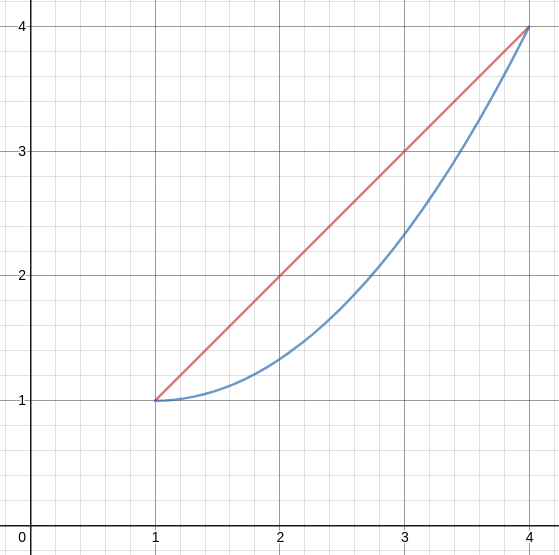
\includegraphics[width=60mm]{images/same_options.png}
  \caption{These two intrinsic options which are considered the same. both start at (1,1) and terminate at (4,4) however their path is different.}
\end{center}
\end{figure}

\pagebreak
Additionally, there are 2 types of options. {\bf Closed loop} options, and {\bf Open loop} options.
\paragraph{Open Loop} options are where you select a sequence of actions to execute and the agent then blindly follows this pre-decided sequence (regardless of new observations).
\paragraph{Closed Loop} options are where you run a policy conditioned on the option representation. This allows the agent to respond to changes in the environment.

\section{Body}

They create an algorithm to generate as many {\bf different options} for an agent as possible. Each of these options should terminate at a different location to all of the others. These options can then be executed by the agent to either maximise reward or maximise ``empowerment'' (which is basically a measure of an agent's ability to reach new states from the current state).


\paragraph{What's so special?} Normally, options are relatively rigid and are simply policies which are learnt by the agent over time, they appear to the agent as actions and return control once they terminate. This paper wants a way to build up a set of options which will allow the agent to get to, or get close to, any state it desires. The point of this paper isn't to make up options which will maximise reward, simply to make up options which will let the agent ``get around''.


\paragraph{What's this about empowerment!?} Using empowerment as an objetive, the agent will seek out states which have the highest number of intrinsic options. Importantly, the agent should be good at actually executing these option policies (otherwise what's the point). Because this is the reinforcement learning paradigm, the agent initially has no understanding of the options which could be available to it, therefore it still needs to explore the environment to find these high empowerment states.


\paragraph{Relationship with unsupervised learning.} In standard UL we have the data likelihood metric for figuring out how good our unsupervised learning algorithm is, we have some data, our UL algorithm identifies some structure and we look at the likelihood to see how well the model explains the data. In the context of this paper we want to do some sort of unsupervised learning to find the intrinsic options available to the agent.


The difference in this case is that with RL, not all the data is known beforehand, the agent needs to interact with the environment to expose examples of different states and environment dynamics.


In RL, instead of using likelihood, the empowerment metric can be used. A higher empowerment suggests our model of the different options is good, since it's basically saying ``our options, with high confidence, will lead to specific final states''.

\begin{equation}
  \label{eq:2}
  \text{Empowerment measures the mutual information between action choices and final states}
\end{equation}

\section{Intrinsic Control}


\end{document}

